\documentclass[10pt]{report}
\makeindex

\usepackage{amsmath, amsfonts, amssymb, amstext, amscd, amsthm, makeidx, graphicx, hyperref, url}
\allowdisplaybreaks

\usepackage{graphicx}
\usepackage{verbatim}
\graphicspath{ {Plots/} }

\setcounter{chapter}{0}
\topmargin -.5in
\addtolength{\hoffset}{-0.6 in}
\addtolength{\textwidth}{1.2 in}
\textheight 9.0in


\begin{document}

\begin{center}\textsc{\Large Ph 20}

\textsc{\large Assignment 3}

\end{center}
Andy Rothstein

\bigskip

\noindent\textbf{Explicit Euler Method}

Initial conditions: $x(0)=0, v(0)=1$.

\includegraphics[scale = .95]{explicit_plot}

To find the analytic solutions to the position and velocity equations, we just need to solve the equation:
$$-kx=\frac{d^2x}{dt^2}.$$
Solving this gives us $x=\sin(t\sqrt k+\phi)$ depending on initial conditions. In our case, we just let $\sqrt k=h$ so that the frequencies of the analytical solution matches the explicit solution. Now when we look at the global error plot between the two plots, we get

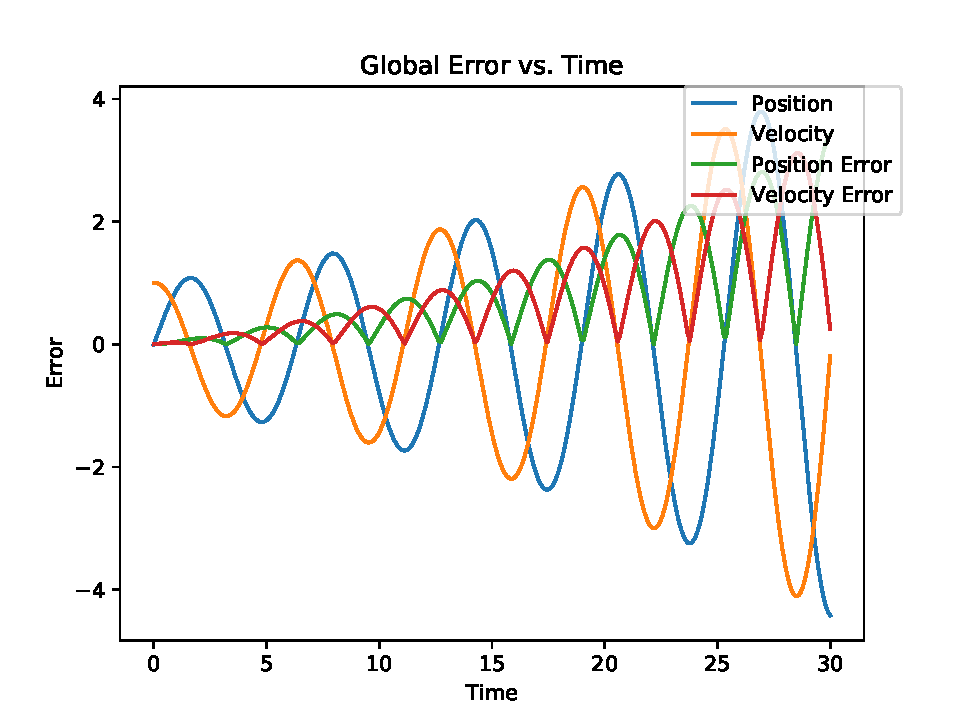
\includegraphics[scale = .85]{error_plot}

Next we see that for small values of $h$, where we take $h=10^{-4}$ to $h=10^{-1}$, we find that the max error produced is linear since it runs parallel to our plot of just a straight line. 

\includegraphics[scale = .85]{h_plot}

\includegraphics[scale = .85]{energy_plot}

From this  energy vs. time plot, we are able to see that the energy in the system increases over time when we use the explicit method to calculate position and velocity. This shows us that we have error in our equations since the error within a closed system like this should not increase in energy over time. 

\noindent\textbf{Implicit Euler Method}

to find the implicit Euler method, we just need to solve the following equation for $x_{i+1}$ and $v_{i+1}$ in terms of $x_i$ and $v_i$:
$$\begin{pmatrix}
1 & -h \\
h & 1 \\
\end{pmatrix}\cdot\begin{pmatrix}
x_{i+1} \\
v_{i+1} \\\end{pmatrix}=\begin{pmatrix}
x_i \\
v_i \\
\end{pmatrix}$$
$$\begin{pmatrix}
x_{i+1} \\
v_{i+1} \\\end{pmatrix}=\frac{1}{1+h^2}\begin{pmatrix}
1 & h \\
-h & 1 \\\end{pmatrix}\cdot\begin{pmatrix}
x_i \\
v_i \\
\end{pmatrix}$$
$$\begin{pmatrix}
x_{i+1} \\
v_{i+1} \\\end{pmatrix}=\frac{1}{1+h^2}\begin{pmatrix}
x_i+hv_i \\
-hx_i+v_i \\\end{pmatrix}$$
Which gives us:
$$x_{i+1}=\frac{x_i+hv_i}{1+h^2}$$
$$v_{i+1}=\frac{v_i-hx_i}{1+h^2}.$$
We can use these equations to plot $x_i$ and $v_i$ vs. time and compare it to the explicit method. We can then create an energy vs. time graph for the implicit method to compare it to the explicit method. 

\includegraphics[scale = .85]{implicit_plot}

\includegraphics[scale = .85]{energy_comp}

Looking at this Energy vs. Time plot that compares both the implicit and explicit methods, we can see that the implicit method will be much more accurate over time compared to the explicit method. The implicit method will be below the actual value, since we are looking for the energy to stay constant at $1$ and the implicit method goes below $1$. 

\includegraphics[scale = .85]{phase_space}

From this phase space geometry diagram, it is clear to see that the explicit and implicit ways of computing the positions and velocities do not conserve the phase space since compared to each other, the explicit spirals out and the implicit spirals in.

\includegraphics[scale = .85]{symp_phase}

From this plot, we can see how the Symplectic Method conserves the phase space since the area of the circle stays constant.

\includegraphics[scale = .85]{symp_energy}

From this comparison of the Symplectic Energy vs the actual energy, we can see that the symplectic energy oscillates sinusoidally compared to the actual energy which just stays constant. 

\bigskip

\textbf{Files}

\textbf{Makefile}
\verbatiminput{Makefile}

\bigskip

\textbf{config.mk}

\verbatiminput{config.mk}

\bigskip

\textbf{energy\_comp.py}

\verbatiminput{energy_comp.py}

\bigskip

\textbf{energy\_plot.py}

\verbatiminput{energy_plot.py}

\bigskip

\textbf{explicit\_plot.py}

\verbatiminput{explicit_plot.py}

\bigskip

\textbf{h\_plot.py}

\verbatiminput{h_plot.py}

\bigskip

\textbf{implicit\_plot.py}

\verbatiminput{implicit_plot.py}

\bigskip

\textbf{phase\_space.py}

\verbatiminput{phase_space.py}

\bigskip

\textbf{symp\_energy.py}

\verbatiminput{symp_energy.py}

\bigskip

\textbf{symp\_phase.py}

\verbatiminput{symp_phase.py}

\bigskip

\textbf{Git Log}

\verbatiminput{log.txt}
 

\end{document}